%% A simple example of how to use the Insight Poster LaTeX Template

% Created 2017-06-20 Tue 12:43 by Sebastian Scheurer
% <sebastian.scheurer@insight-centre.org> at (and for) the Insight
% Centre for Data Analytics, Dep. of Computer Science, University
% College Cork, Cork, Ireland.

\documentclass[presentation,17pt]{beamer}
\usepackage[orientation=portrait,size=a0,scale=1.4]{beamerposter}

\usepackage{tabularx}
\usepackage[square,numbers,sort]{natbib}
\usepackage{ragged2e}

\setbeamertemplate{caption}[numbered]

% This loads the insight template from file beamerInsightPoster.sty,
% which must be somewhere LaTeX can find it. The easiest thing to do
% is to put everything in the same folder as your poster.
\usetheme{InsightPoster17}

\author{\texorpdfstring{Nivranshu Pasricha \and Conor Hayes \newline\url{nivranshu.pasricha@insight-centre.org}}{Author}}

% If you use a PDF-aware LaTeX processor this is stored as the PDF
% title, but is invisible on the poster itself.
\title{AICS Poster}

% Acknowledge funding here. This command *must* be used after
% ``\usetheme{InsightPoster17}''.
\insightFundingBy{This work has emanated from research supported in part by a research grant from Science Foundation Ireland (SFI) under Grant Number SFI/12/RC/2289P2.}

\setbeamertemplate{background}{
  % You can change this if the poster_background_2017.pdf is not in the
  % same folder as your poster.
  
\includegraphics[width=\paperwidth,height=\paperheight]{poster_background_2017.pdf}
}

\begin{document}
%%%%%%%%%%%%%%%%%%%%%%%%%%%%%%%%%%%%%%%%%%%%%%%%%%%%%%%%%%%%%%%%%%%%%%%
%                             BEGIN POSTER                            %

% The frame environment is your poster. So go ahead and replace those
% \blind<text|itemize|enumerate|description> items with your own
% content.
% \begin{frame}{Insert print title here: \LaTeX\ will wrap and hyphenate it as needed}
\begin{frame}{Detecting Bot Behaviour \\ in Social Media using \\ Digital DNA Compression}
  \begin{columns}[t]


    %%%%%%%%%%%%%%%%%%%%%%%%%%%%%%%%%%
    %       BEGIN LEFT COLUMN        %
    \begin{column}{0.48\textwidth}
      \begin{block}{Introduction}
        \justifying{It is estimated that bots make up 9-15\% of all Twitter accounts. A paradigm-shift \cite{Cresci:2017:PSS:3041021.3055135} has been observed in the last few years in the behaviour of Twitter bots where more sophisticated social bots have been identified that can fool traditional bot detection techniques as well as human annotators.}
      \end{block}

      \begin{block}{Digital DNA}
        \justifying{We assume that the long-term behaviour of a bot account is less random than the behaviour of a genuine user and we model the temporal activity \cite{Kan2013} of a Twitter account using the technique of digital DNA \cite{7876716} with the following alphabet: \\ }
            \[ 
                \mathbf{B}^{3}_{type} = 
                \left \{
                  \begin{tabular}{l}
                  $\texttt{A} \leftarrow \textrm{tweet}, $ \\
                  $\texttt{C} \leftarrow \textrm{reply}, $ \\
                  $\texttt{T} \leftarrow \textrm{retweet} $
                  \end{tabular}
                \right \}
            \]
        \end{block}
        \begin{block}{String Compression}
          \justifying{A string \texttt{s} $=$ ``\texttt{ACTCATTTTA}" can represent a sequence of 10 posts made by an account. We employ a string compression algorithm on such digital DNA sequences and use the compression statistics as features to train a logistic regression model that classifies Twitter accounts as bots or genuine users.}
        
        \begin{figure}
          \caption{Compression statistics for Digital DNA sequences.}
          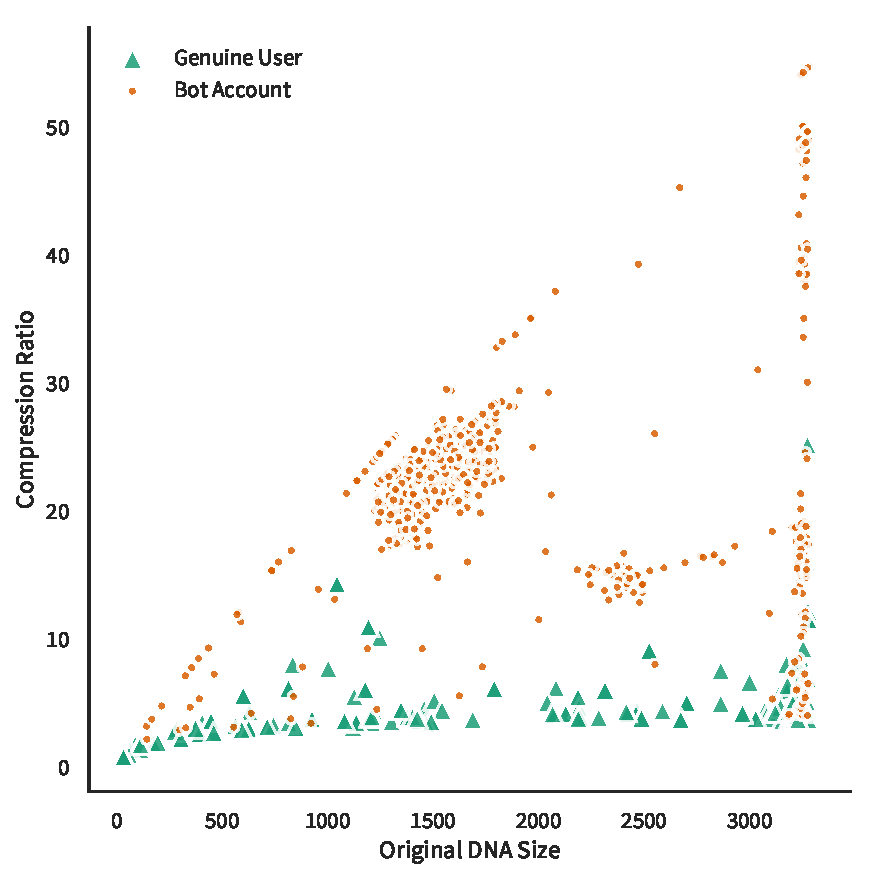
\includegraphics[width=0.7\linewidth]{dna-scatter-2.pdf}
        \end{figure}
        
      \end{block}
    \end{column}
    %        END LEFT COLUMN         %
    %%%%%%%%%%%%%%%%%%%%%%%%%%%%%%%%%%

    %%%%%%%%%%%%%%%%%%%%%%%%%%%%%%%%%%
    %  BEGIN MIDDLE (EMPTY) COLUMN   %
    \begin{column}{0.04\textwidth}
    \end{column}
    %    END MIDDLE (EMPTY) COLUMN   %
    %%%%%%%%%%%%%%%%%%%%%%%%%%%%%%%%%%

    %%%%%%%%%%%%%%%%%%%%%%%%%%%%%%%%%%
    %       BEGIN RIGHT COLUMN       %
    \begin{column}{0.48\textwidth}
      \begin{block}{Length of Digital DNA Sequence}
        \justifying{We set different limits $L = \{10, 25, 50, 100, 200, 500, 1000, 2000\} $ for the maximum length of the DNA sequence and for each account, we pick a DNA sub-sequence of random length between $1$ and $L$. We observe great improvements in the performance as the DNA sequence length increases. }
        \begin{figure}
          \caption{Results with different values for maximum sequence length $L$.}
          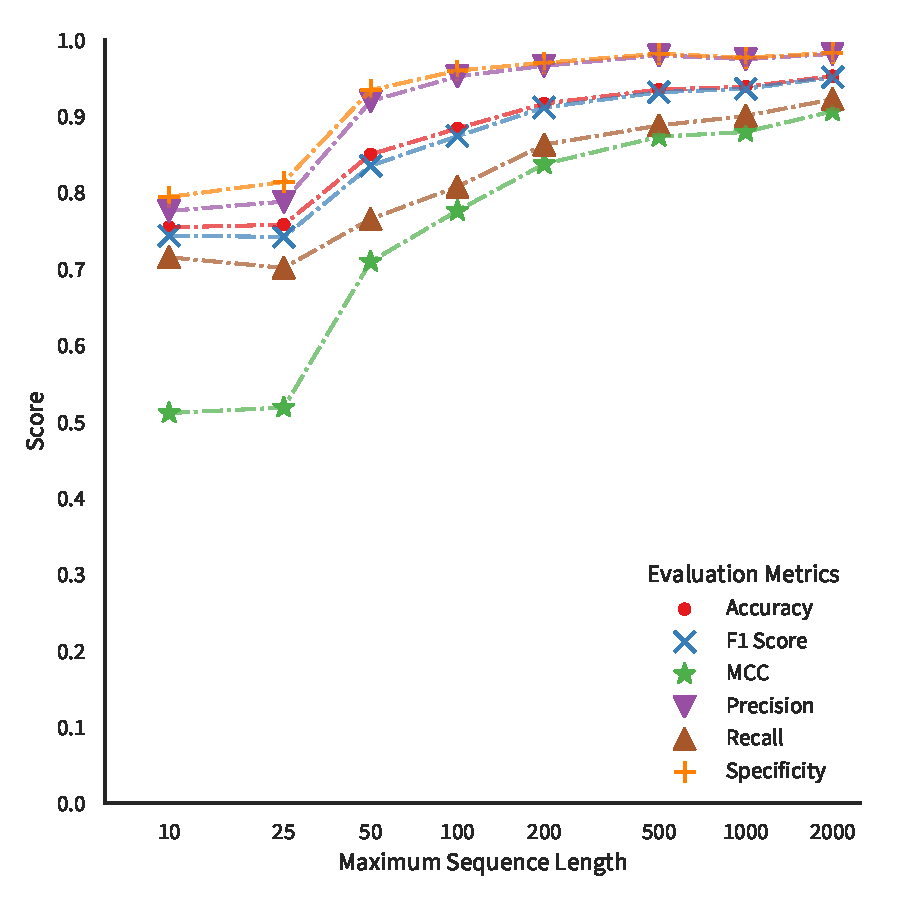
\includegraphics[width=0.7\linewidth]{dna-len-1.pdf}
        \end{figure}
      \end{block}
      
      \begin{block}{Conclusion \& Future Work}
        \justifying{Our approach is a fast and scalable extension on the idea of digital DNA, which is language and content independent as well as easy to represent visually. Future work can incorporate other user-profile and content-based features into the digital DNA sequence and apply this technique to identify automated accounts on other social media platforms such as Facebook and Reddit.}
      \end{block}

      \begin{block}{References}
        \small{
          \bibliographystyle{abbrvnat}
          \bibliography{biblio.bib}
        }
      \end{block}
    \end{column}
    %        END RIGHT COLUMN        %
    %%%%%%%%%%%%%%%%%%%%%%%%%%%%%%%%%%
    
  \end{columns} % End column environment.


  \begin{block}{Results}
    \begin{table}
      \caption{\label{tab:eval} Comparison of our bot detection technique based on String Compression with the k-Common Substring technique from \cite{7876716}. The dataset contains a random sample of genuine user accounts and a sample of bot accounts which were found to be created to target Mayoral elections in Rome, Italy.}
      \begin{tabularx}{\textwidth}{{X}*{7}{c}}
        \hline
        \multicolumn{1}{c}{Technique} &
        \multicolumn{6}{c}{Metrics} \\
        \hline
        & {Accuracy} & {Precision} & {Recall} & {F-Measure} & {MCC} & {Specificity} \\
        \hline
        k-Common Substring - Unsupervised \cite{7876716} & 0.976 & 0.982 & 0.972 & 0.977 & 0.952 & 0.981 \\
        k-Common Substring - Supervised \cite{7876716} & 0.977 & 0.982 & 0.977 & 0.977 & 0.955 & 0.981 \\
        \textbf{String Compression - Compressed DNA Size} & \textbf{0.980} & 0.978 & \textbf{0.981} & \textbf{0.980} & \textbf{0.960} & 0.978 \\
        \textbf{String Compression - Compression Ratio} & \textbf{0.984} & \textbf{0.992} & 0.976 & \textbf{0.984} & \textbf{0.968} & \textbf{0.992} \\
        \hline
      \end{tabularx}
    \end{table}
  \end{block}
  
\end{frame}
%                             END POSTER                               %
%%%%%%%%%%%%%%%%%%%%%%%%%%%%%%%%%%%%%%%%%%%%%%%%%%%%%%%%%%%%%%%%%%%%%%%%

\end{document}
